\question Give a tight bound on the overall runtime of the following function


\begin{lstlisting}
int f(int N) {
	if (N == 1) 
		return 1;
	int y = 0;
	for (int x = 0; x < N; x += 1) {
		y += 1;
	}
	return f(N/2) + f(N/2) + y;
} 

\end{lstlisting}

\begin{solution}[1.5in]
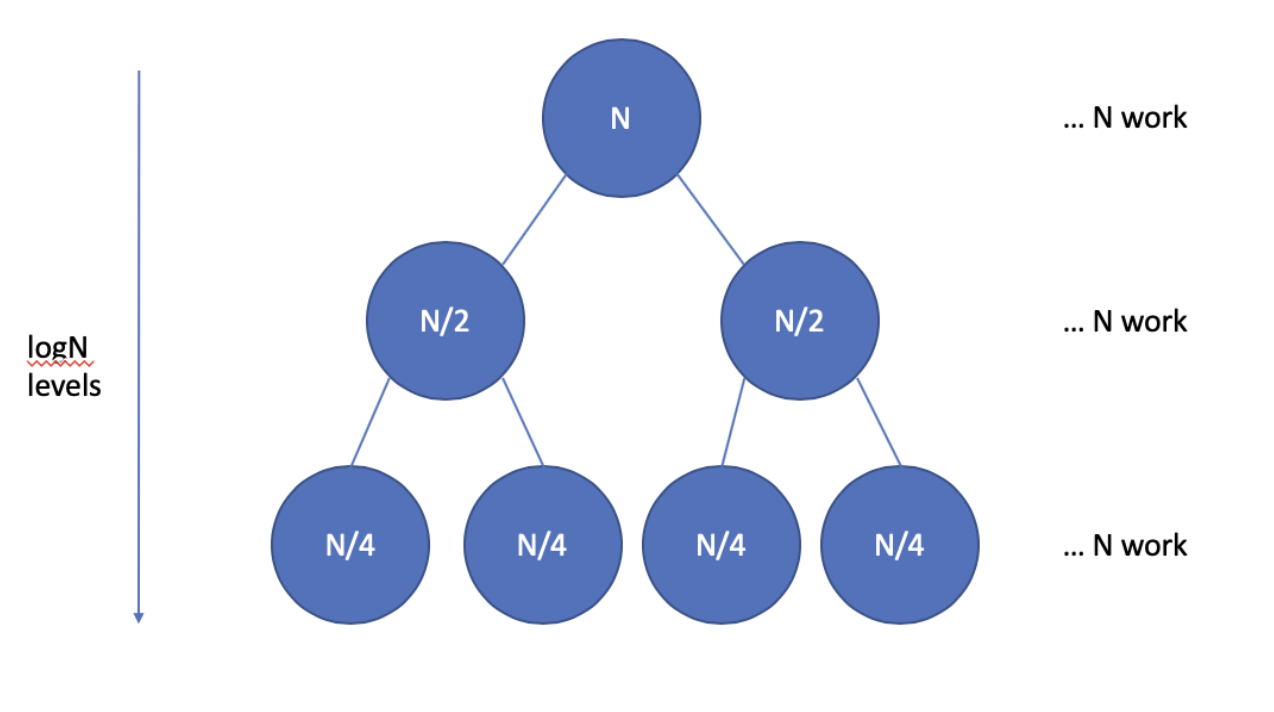
\includegraphics[scale=0.35]{topics/asymptotics/MockMidterm/RuntimeTree.png}

The branching factor at each node is two because on each function call, 2 recursive calls are made. Due to the for loop, each function does a linear amount of work with respect to its argument. This is represented in the tree through the value in each of the nodes. There are logN levels since N is divided by two on each recursive call. Since there are logN levels and each level does a total of N work, the upper and lower bounds are $O(N\log N)$ and $\Omega(N\log N)$ respectively. Since those have the same runtime, they converge to a $\Theta$ bound of $\Theta(N\log N)$.

\end{solution}